\documentclass{beamer}
\usepackage{tikz,amsmath,hyperref,graphicx,stackrel,animate}
\usetikzlibrary{positioning,shadows,arrows,shapes,calc}
\newcommand{\argmax}{\operatornamewithlimits{argmax}}
\newcommand{\argmin}{\operatornamewithlimits{argmin}}
\mode<presentation>{\usetheme{Frankfurt}}
\AtBeginSection[]
{
  \begin{frame}<beamer>
    \frametitle{Outline}
    \tableofcontents[currentsection,currentsubsection]
  \end{frame}
}
\title{Lecture 12: Principal Components and Eigenfaces}
\author{Mark Hasegawa-Johnson\\All content~\href{https://creativecommons.org/licenses/by/4.0/}{CC-BY 4.0} unless otherwise specified.}
\date{ECE 417: Multimedia Signal Processing, Fall 2021}  
\begin{document}

% Title
\begin{frame}
  \maketitle
\end{frame}

% Title
\begin{frame}
  \tableofcontents
\end{frame}

%%%%%%%%%%%%%%%%%%%%%%%%%%%%%%%%%%%%%%%%%%%%
\section[Review]{Review: Gaussians}
\setcounter{subsection}{1}

\begin{frame}
  \frametitle{Scalar Gaussian random variables}
  \[
  p_X(x) = \frac{1}{\sqrt{2\pi\sigma^2}}e^{-\frac{1}{2}\left(\frac{x-\mu}{\sigma}\right)^2}
  \]
  \centerline{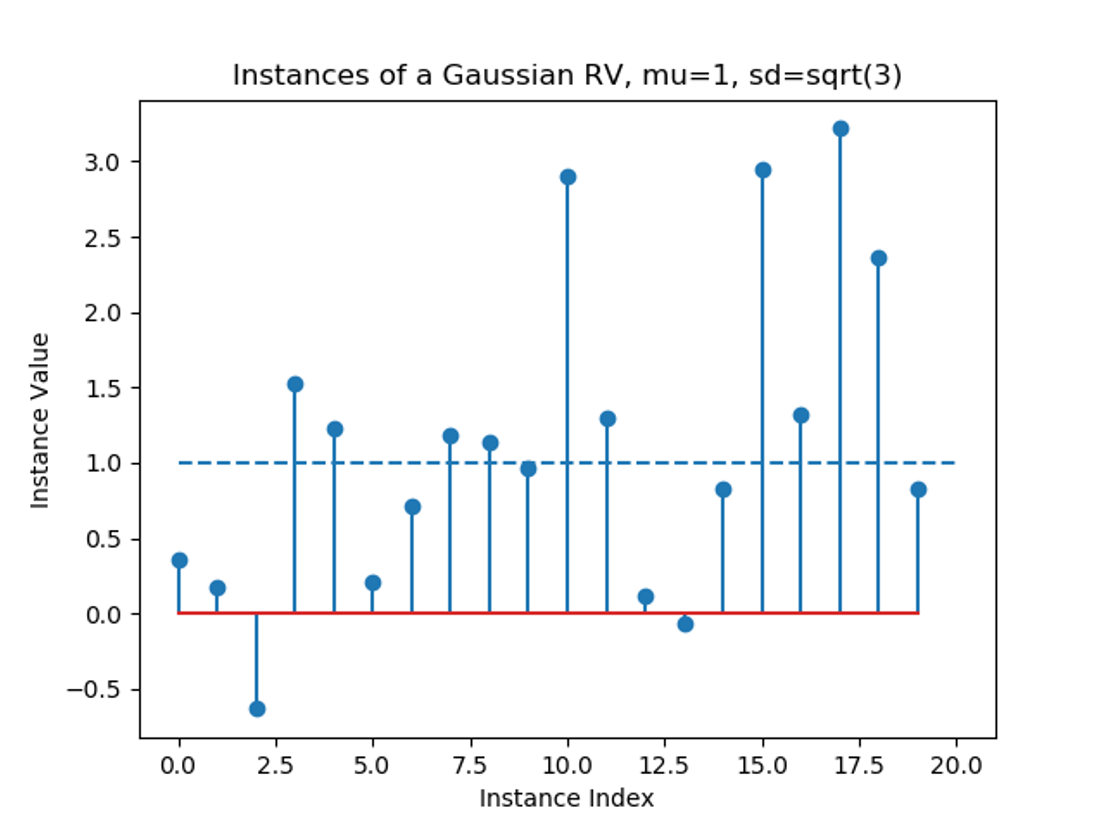
\includegraphics[height=3in]{gaussian_instances.png}}
\end{frame}

\begin{frame}
  \frametitle{Scalar Gaussian random variables}
  \[
  \mu=E[X],~~~\sigma^2=E[(X-\mu)^2]
  \]
  \centerline{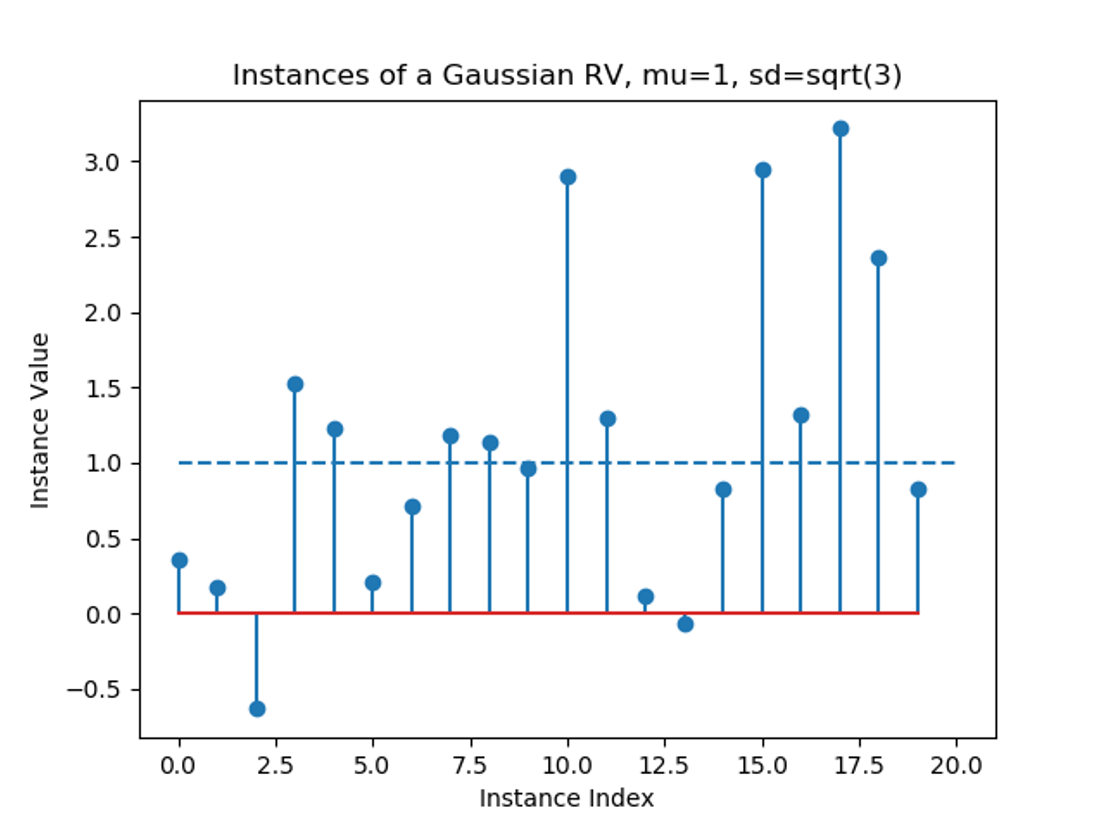
\includegraphics[height=3in]{gaussian_instances.png}}
\end{frame}

\begin{frame}
  \frametitle{Gaussian random vector}
  \[
  p_{\vec{X}}(\vec{x})=\frac{1}{(2\pi)^{D/2}|\Sigma|^{1/2}}e^{-\frac{1}{2}
    (\vec{x}-\vec\mu)^T\Sigma^{-1}(\vec{x}-\vec\mu)}
  \]
  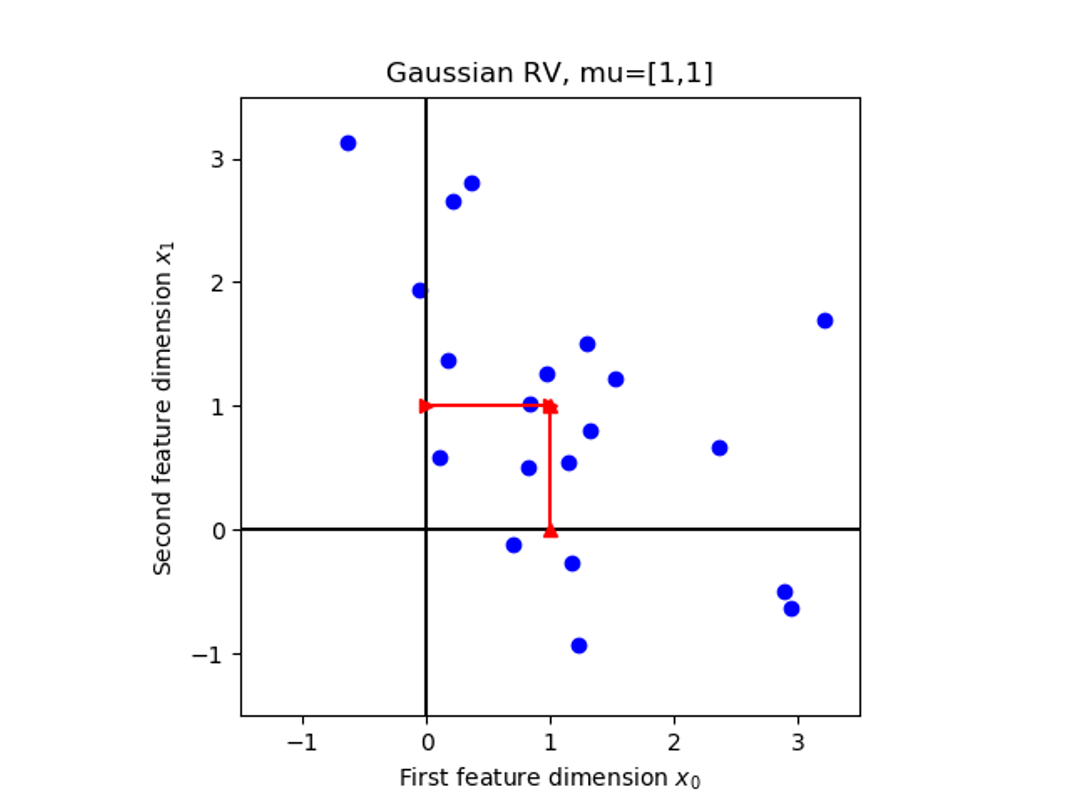
\includegraphics[width=2.1in]{gaussian_vectors.png}
\end{frame}

\begin{frame}
  \begin{columns}
    \column{2.125in}
    \begin{block}{Gaussian random vector}
      \[
      \vec{x}=\left[\begin{array}{c}x_0\\\cdots\\x_{D-1}\end{array}\right]
      \]
      \[
      \vec\mu=E[\vec{x}]=\left[\begin{array}{c}\mu_0\\\cdots\\\mu_{D-1}\end{array}\right]
      \]
    \end{block}
    \column{2.125in}
    \begin{block}{Example: Instances of a Gaussian random vector}
      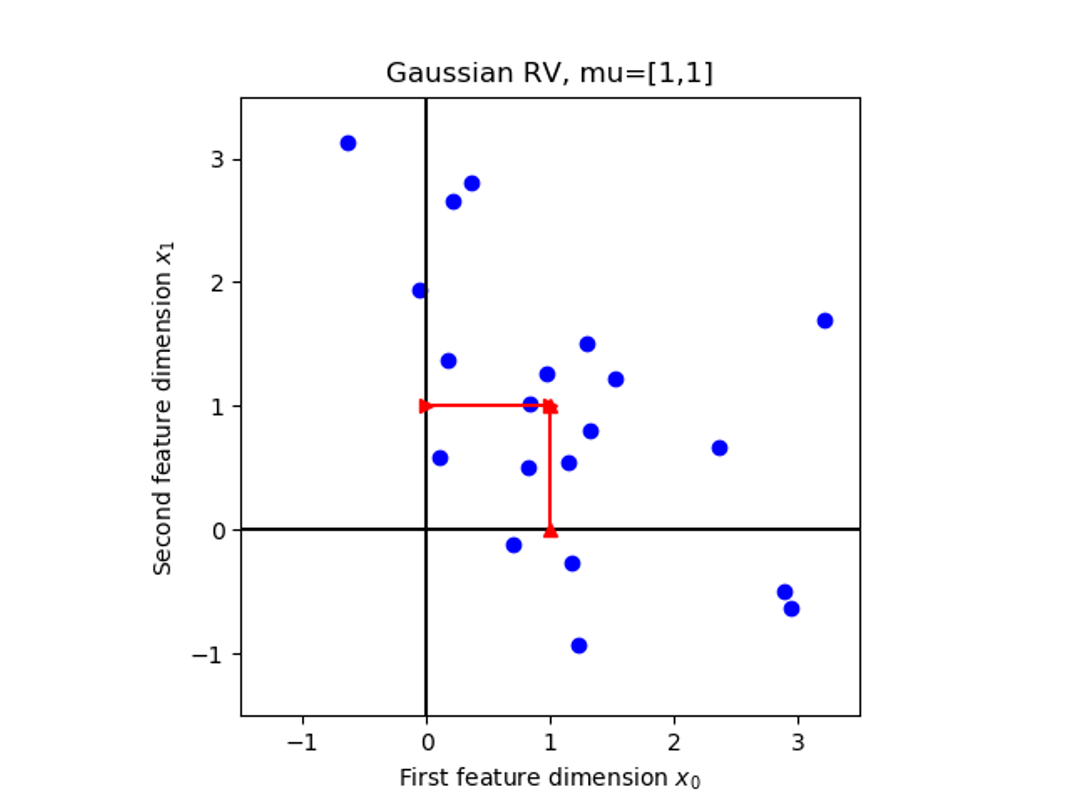
\includegraphics[width=2.1in]{gaussian_vectors.png}
    \end{block}
  \end{columns}
\end{frame}

\begin{frame}
  \begin{columns}
    \column{2.25in}
    \begin{block}{Gaussian random vector}
      \[
      \Sigma= \left[\begin{array}{ccc}
          \sigma_0^2 & \rho_{0,1} & \ddots\\
          \rho_{1,0} & \ddots &  \rho_{D-2,D-1}\\
          \ddots & \rho_{D-1,D-2} &  \sigma_{D-1}^2\end{array}\right]
      \]
      where
      \[
      \rho_{ij}=E[(x_i-\mu_i)(x_j-\mu_j)]
      \]
      \[
      \sigma_{i}^2=E[(x_i-\mu_i)^2]
      \]
    \end{block}
    \column{2in}
    \begin{block}{Example: Instances of a Gaussian random vector}
      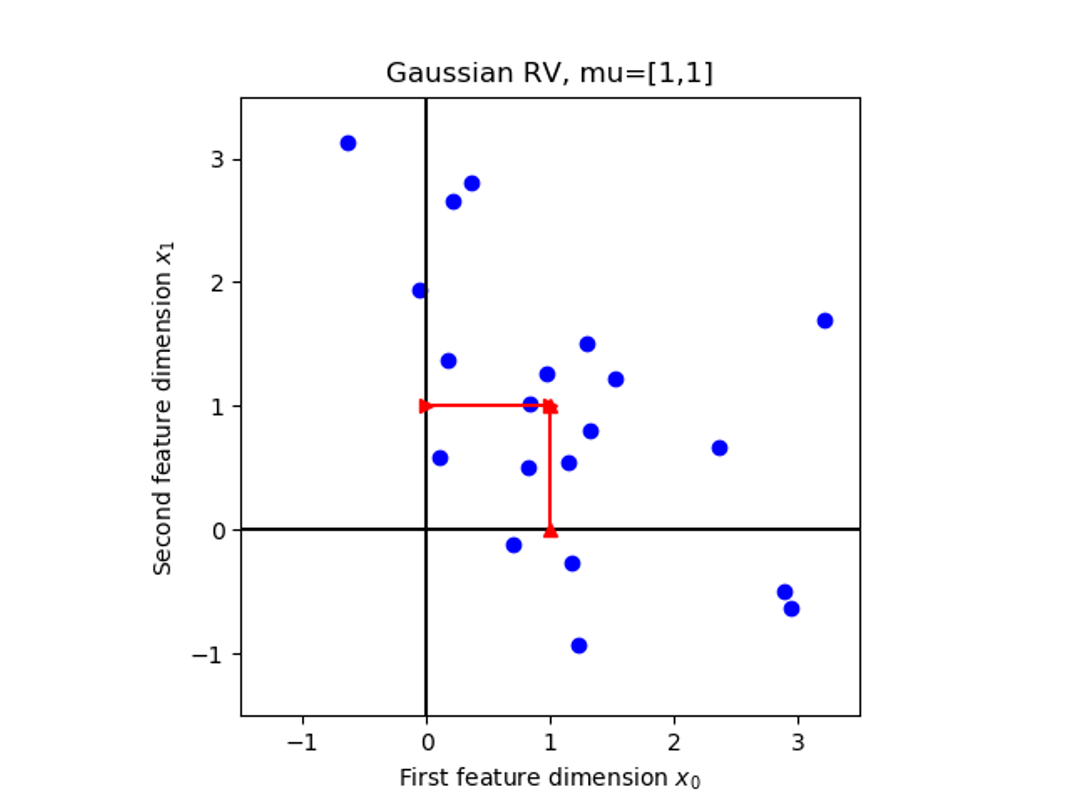
\includegraphics[width=1.9in]{gaussian_vectors.png}
    \end{block}
  \end{columns}
\end{frame}

\begin{frame}
  \begin{columns}
    \column{2.25in}
    \begin{block}{Maximum Likelihood Parameter Estimation}
      In the real world, we don't know $\vec\mu$ and $\Sigma$!

      If we have a training database ${\mathcal
        D}=\left\{\vec{x}_0,\ldots,\vec{x}_{M-1}\right\}$, we can
      estimate $\vec\mu$ and $\Sigma$ according to
      \begin{align*}
        \left\{\hat\mu_{ML},\hat{\Sigma}_{ML}\right\} &= \argmax
        \prod_{m=0}^{M-1} p(\vec{x}_m|\vec\mu,\Sigma)\\
        &= \argmax
        \sum_{m=0}^{M-1} \ln p(\vec{x}_m|\vec\mu,\Sigma)
      \end{align*}
    \end{block}
    \column{2in}
    \begin{block}{Examples of $\vec{x}_m-\vec\mu$}
      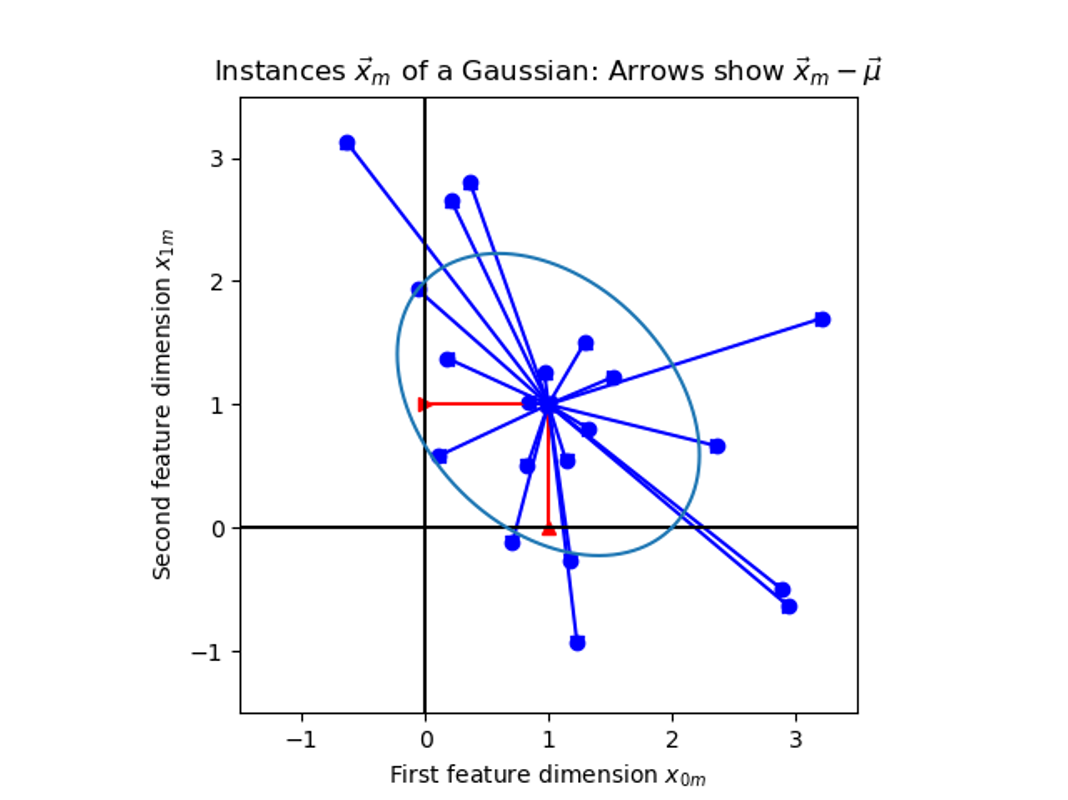
\includegraphics[width=1.9in]{gaussian_subtraction.png}
    \end{block}
  \end{columns}
\end{frame}

\begin{frame}
  \begin{columns}
    \column{2.25in}
    \begin{block}{Maximum Likelihood Parameter Estimation}
      If you differentiate the RHS on the previous slide, and set it
      to zero, you find that the maximum likelihood solution is
      \begin{align*}
        \hat{\mu}_{ML} &= \frac{1}{M}\sum_{m=0}^{M-1}\vec{x}_m\\
        \hat{\Sigma}_{ML} &= \frac{1}{M}\sum_{m=0}^{M-1}(\vec{x}_m-\vec\mu)(\vec{x}_m-\vec\mu)^T
      \end{align*}
    \end{block}
    \column{2in}
    \begin{block}{Examples of $\vec{x}_m-\vec\mu$}
      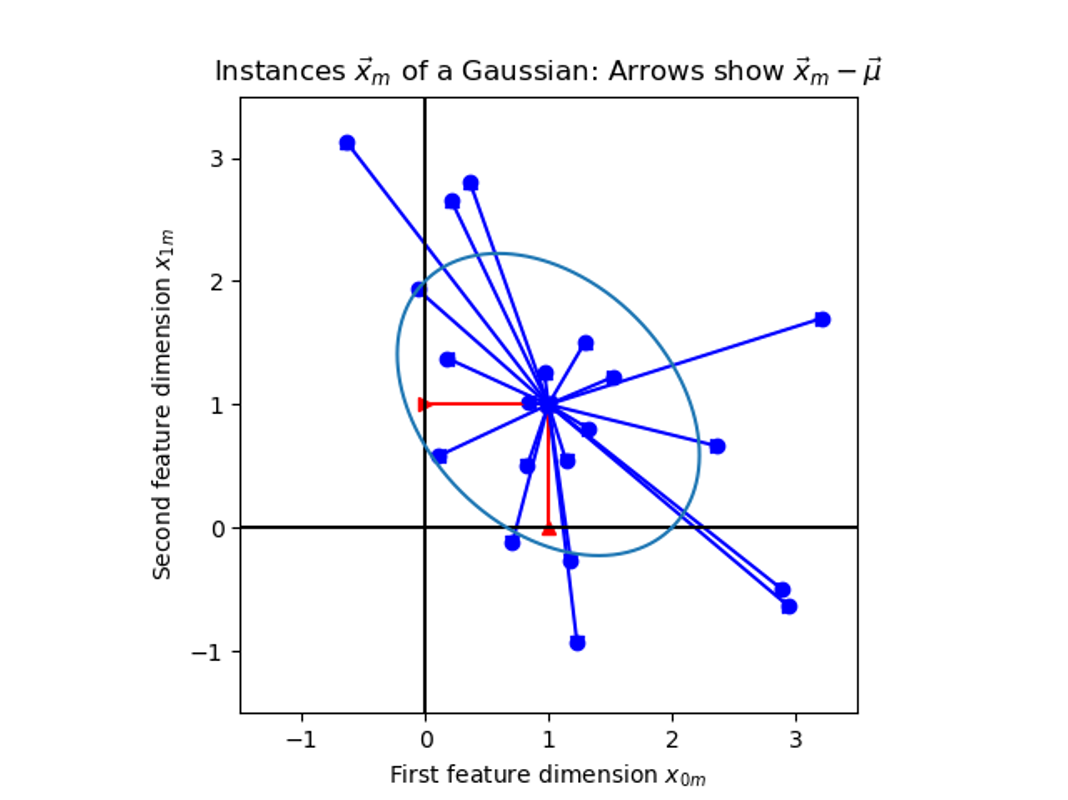
\includegraphics[width=1.9in]{gaussian_subtraction.png}
    \end{block}
  \end{columns}
\end{frame}

\begin{frame}
  \begin{columns}
    \column{2.25in}
    \begin{block}{Sample Mean, Sample Covariance}
      The ML estimate of $\Sigma$ is usually too small.  It is better
      to adjust it slightly.  The following are the {\bf unbiased
        estimators} of $\vec\mu$ and $\Sigma$, also called the {\bf
        sample mean} and {\bf sample covariance}:
      \[
      \vec\mu=\frac{1}{M}\sum_{m=0}^{M-1}\vec{x}_m
      \]
      \[
      \Sigma=\frac{1}{M-1}\sum_{m=0}^{M-1}(\vec{x}_m-\vec\mu)(\vec{x}_m-\vec\mu)^T
      \]
    \end{block}
    \column{2in}
    \begin{block}{Examples of $\vec{x}_m-\vec\mu$}
      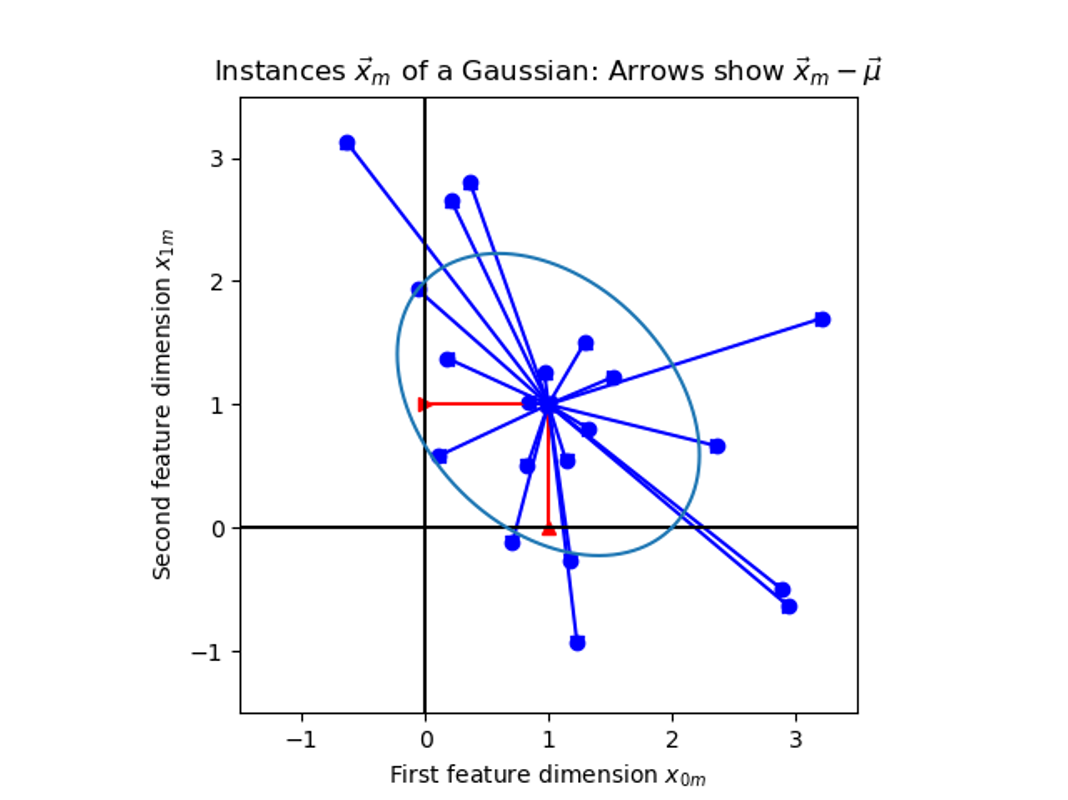
\includegraphics[width=1.9in]{gaussian_subtraction.png}
    \end{block}
  \end{columns}
\end{frame}

\begin{frame}
  \begin{columns}
    \column{2.25in}
    \begin{block}{Sample Mean, Sample Covariance}
      \[
      \vec\mu=\frac{1}{M}\sum_{m=0}^{M-1}\vec{x}_m
      \]
      \[
      \Sigma=\frac{1}{M-1}\sum_{m=0}^{M-1}(\vec{x}_m-\vec\mu)(\vec{x}_m-\vec\mu)^T
      \]
      Sample mean and sample covariance are not the same as real mean
      and real covariance, but we'll use the same letters ($\vec\mu$
      and $\Sigma$) unless the problem requires us to distinguish.
    \end{block}
    \column{2in}
    \begin{block}{Examples of $\vec{x}_m-\vec\mu$}
      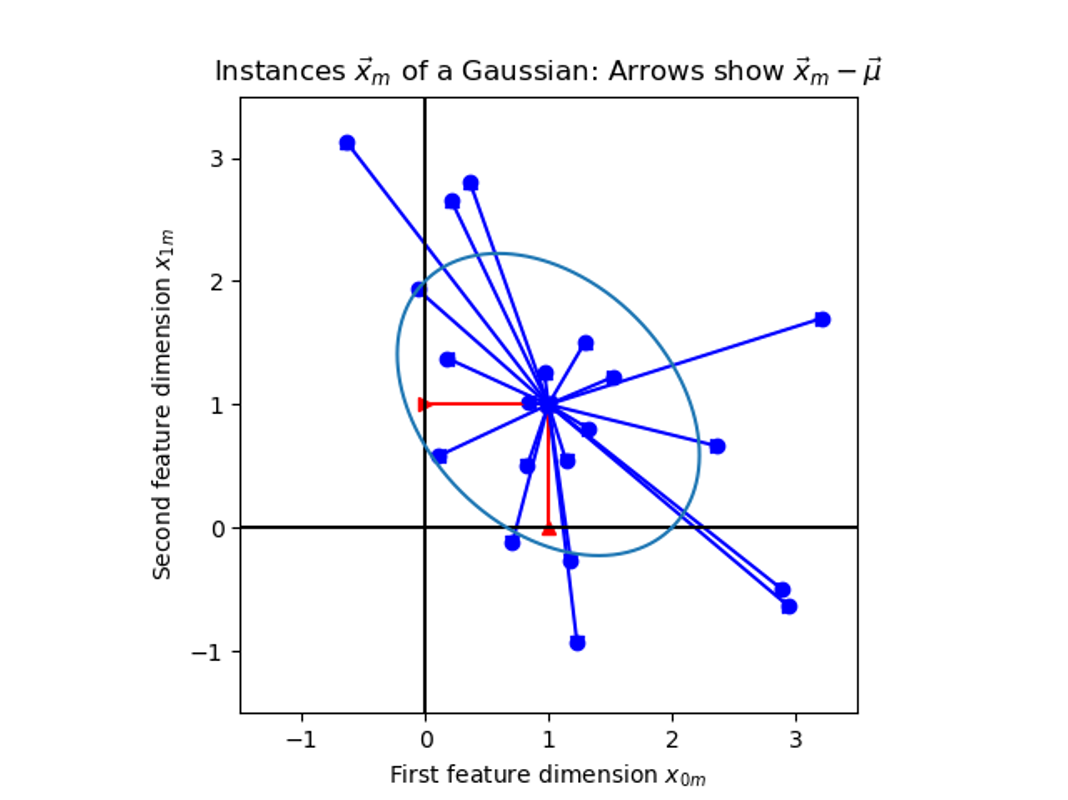
\includegraphics[width=1.9in]{gaussian_subtraction.png}
    \end{block}
  \end{columns}
\end{frame}

%%%%%%%%%%%%%%%%%%%%%%%%%%%%%%%%%%%%%%%%%%%%
\section[Eigenvectors]{Review: Eigenvectors}
\setcounter{subsection}{1}


\begin{frame}
  \frametitle{Review: Eigenvalues and eigenvectors}
  The right eigenvectors of a $D\times D$ square matrix, $A$, are the
  vectors $\vec{v}$ such that
  \begin{equation}
    A\vec{v}=\lambda\vec{v}
    \label{eq:eigenvectors}
  \end{equation}
  The scalar, $\lambda$, is called the eigenvalue.  It's only possible
  for Eq.~(\ref{eq:eigenvectors}) to have a solution if
  \begin{equation}
    |A-\lambda I|=0
    \label{eq:eigenvalues}
  \end{equation}
\end{frame}

\begin{frame}
  \frametitle{Left and right eigenvectors}
  We’ve been working with right eigenvectors and right eigenvalues: 
  \[
  A\vec{v}_d =\lambda_d\vec{v}_d
  \]
  There may also be left eigenvectors, which are row vectors $\vec{u}_d$
  and corresponding left eigenvalues $\kappa_d$:
  \[
  \vec{u}_d^T A = \kappa_d\vec{u}_d^T
  \]
\end{frame}

\begin{frame}
  \frametitle{Eigenvectors on both sides of the matrix}
  You can do an interesting thing if you multiply the matrix by its eigenvectors both before and after:
  \[
  \vec{u}_i^T(A\vec{v}_j)=\vec{u}_i^T(\lambda_j\vec{v}_j)=\lambda_j\vec{u}_i^T\vec{v}_j
  \]
  \ldots but\ldots
  \[
  (\vec{u}_i^TA)\vec{v}_j=(\kappa_i\vec{u}_i^T)\vec{v}_j=\kappa_i\vec{u}_i^T\vec{v}_j
  \]
  There are only two ways that both of these things can be true. Either
  \[
  \kappa_i=\lambda_j~~~\mbox{or}~~~\vec{u}_i^T\vec{v}_j=0
  \]
\end{frame}

\begin{frame}
  \frametitle{Left and right eigenvectors must be paired!!}
  There are only two ways that both of these things can be true. Either
  \[
  \kappa_i=\lambda_j~~~\mbox{or}~~~\vec{u}_i^T\vec{v}_j=0
  \]
  That means, if the eigenvalues are {\bf distinct}, then there is
  {\bf at most one} $\lambda_i$ that can equal each $\kappa_i$:
  \[
  \begin{cases}
    i\ne j & \vec{u}_i^T\vec{v}_j = 0\\
    i=j & \kappa_i = \lambda_i
  \end{cases}
  \]
\end{frame}

\begin{frame}
  \frametitle{Symmetric matrices: left=right}

  If $A$ is symmetric ($A=A^T$), then the left and right eigenvectors
  and eigenvalues are the same, because
  \[
  \lambda_i\vec{u}_i^T=\vec{u}_i^TA=(A^T\vec{u}_i)^T=(A\vec{u}_i)^T
  \]
  $\ldots$ and that last term is equal to $\lambda_i\vec{u}_i^T$ if and
  only if $\vec{u}_i=\vec{v}_i$.
\end{frame}

\begin{frame}
  \frametitle{Symmetric matrices: eigenvectors are orthonormal}
  Let's combine the following facts:
  \begin{itemize}
  \item $\vec{u}_i^T\vec{v}_j=0$ for $i\ne j$ --- any square matrix with distinct
    eigenvalues
  \item $\vec{u}_i=\vec{v}_i$ --- symmetric matrix
  \item $\vec{v}_i^T\vec{v}_i=1$ --- standard normalization of
    eigenvectors for any matrix (this is what $\Vert\vec{v}_i\Vert=1$ means).
  \end{itemize}
  Putting it all together, we get that
  \[
  \vec{v}_i^T\vec{v}_j=
  \begin{cases}
    1&i=j\\
    0&i\ne j
  \end{cases}
  \]
\end{frame}

\begin{frame}
  \frametitle{The eigenvector matrix}
  So if $A$ is symmetric with distinct eigenvalues, then
  its eigenvectors  are orthonormal:
  \[
  \vec{v}_i^T\vec{v}_j=
  \begin{cases}
    1&i=j\\
    0&i\ne j
  \end{cases}
  \]
  We can  write this as
  \[
  V^TV = I
  \]
  where
  \[
  V=\left[\vec{v}_0,\ldots,\vec{v}_{D-1}\right]
  \]
\end{frame}

\begin{frame}
  \frametitle{The eigenvector matrix is orthonormal}
  \[
  V^TV = I
  \]
  \ldots and it also turns out that
  \[
  VV^T = I
  \]
  Proof: 
  $VV^T=VIV^T=V(V^TV)V^T=(VV^T)^2$, but the only matrix that satisfies
  $VV^T=(VV^T)^2$ is $VV^T=I$.
\end{frame}

\begin{frame}
  \frametitle{Eigenvectors orthogonalize a symmetric matrix}
  So now, suppose $A$ is symmetric:
  \[
  \vec{v}_i^TA\vec{v}_j=
  \vec{v}_i^T(\lambda_j\vec{v}_j)=\lambda_j\vec{v}_i^T\vec{v}_j
  =\begin{cases}\lambda_j,&i=j\\0,&i\ne j\end{cases}
  \]
  In other words, if a symmetric matrix has $D$ eigenvectors with
  distinct eigenvalues, then its eigenvectors orthogonalize $A$:
  \[
  V^TAV = \Lambda
  \]
  \[
  \Lambda=
  \left[\begin{array}{ccc}\lambda_0&0&0\\0&\ldots&0\\0&0&\lambda_{D-1}\end{array}\right]
  \]
\end{frame}

\begin{frame}
  \frametitle{A symmetric matrix is the weighted sum of its eigenvectors:}
  One more thing.  Notice that
  \[
  A = VV^TAVV^T =V\Lambda V^T
  \]
  The last term is
  \[
  \left[\vec{v}_0,\ldots,\vec{v}_{D-1}\right]
  \left[\begin{array}{ccc}\lambda_0&0&0\\0&\ldots&0\\0&0&\lambda_{D-1}\end{array}\right]  
  \left[\begin{array}{c}\vec{v}_0^T\\\vdots\\\vec{v}_{D-1}^T\end{array}\right]=
  \sum_{d=0}^{D-1}\lambda_d \vec{v}_d\vec{v}_d^T
  \]
\end{frame}

\begin{frame}
  \frametitle{Summary: properties of symmetric matrices}
  If $A$ is symmetric with $D$ eigenvectors, and $D$ distinct eigenvalues, then
  \[
  A=V\Lambda V^T
  \]
  \[
  \Lambda = V^TAV
  \]
  \[
  VV^T=V^TV=I
  \]
\end{frame}


%%%%%%%%%%%%%%%%%%%%%%%%%%%%%%%%%%%%%%%%%%%%
\section[NN]{Nearest-Neighbors Classifier}
\setcounter{subsection}{1}

\begin{frame}
  \frametitle{How do you classify an image?}

  Suppose we have a test image, $\vec{x}_{\mbox{test}}$.  We want to figure out:
  who is this person?

  \begin{centering}
    \begin{block}{\bf Test Datum $\vec{x}_{\mbox{test}}$:}
      
\includegraphics[width=1.5in]{exp/Megawati_Sukarnoputri_0002.jpg}
    \end{block}
  \end{centering}
  
\end{frame}
    
\begin{frame}
  \frametitle{Training Data?}
  In order to classify the test image, we need some training data.
  For example, suppose we have the following four images in our
  training data.  Each image, $\vec{x}_m$, comes with a label, $y_m$,
  which is just a string giving the name of the individual.
  \begin{columns}
    \column{1.05in}
    \begin{block}{\bf Training Datum: $y_0=$Colin Powell:}
      $\vec{x}_0=$
      
\includegraphics[width=1in]{exp/Colin_Powell_0001.jpg}
    \end{block}
    \column{1.05in}
    \begin{block}{\bf Training Datum $y_1=$Gloria Arroyo:}
      $\vec{x}_1=$
      
\includegraphics[width=1in]{exp/Gloria_Macapagal_Arroyo_0001.jpg}
    \end{block}
    \column{1.05in}
    \begin{block}{\bf Training Datum $y_2=$Megawati Sukarnoputri:}
      $\vec{x}_2=$
      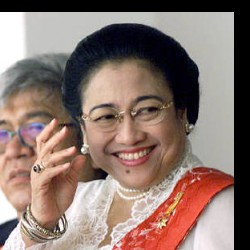
\includegraphics[width=1in]{exp/Megawati_Sukarnoputri_0001.jpg}
    \end{block}
    \column{1.05in}
    \begin{block}{\bf Training Datum $y_3=$Tony Blair:}
      $\vec{x}_3=$
      
\includegraphics[width=1in]{exp/Tony_Blair_0001.jpg}
    \end{block}
  \end{columns}
\end{frame}
    
\begin{frame}
  \frametitle{Nearest Neighbors Classifier}

  A ``nearest neighbors classifier'' makes the following
  guess: the test vector is an image of the same person as the
  closest training vector:
  \[
  \hat{y}_{\mbox{test}} = y_{m^*},~~~
  m^*=\argmin_{m=0}^{M-1}\Vert\vec{x}_m-\vec{x}_{\mbox{test}}\Vert
  \]
  where ``closest,'' here, means Euclidean distance:
  \[
  \Vert\vec{x}_m-\vec{x}_{\mbox{test}}\Vert =
  \sqrt{\sum_{d=0}^{D-1} (x_{md}-x_{\mbox{test},d})^2}
  \]
\end{frame}

\begin{frame}
  \frametitle{Improved Nearest Neighbors: Eigenface}

  \begin{itemize}
    \item 
      The problem with nearest-neighbors is that subtracting one image
      from another, pixel-by-pixel, results in a measurement that is
      dominated by noise.
    \item 
      We need a better measurement.
    \item
      The solution is to find a signal representation, $\vec{y}_m$,
      such that $\vec{y}_m$ summarizes the way in which $\vec{x}_m$
      differs from other faces.
    \item
      If we find $\vec{y}_m$ using principal components analysis, then
      $\vec{y}_m$ is called an ``eigenface'' representation.
  \end{itemize}
\end{frame}
  

%%%%%%%%%%%%%%%%%%%%%%%%%%%%%%%%%%%%%%%%%%%%
\section[PCA]{Today's key point: Principal components = Eigenfaces}
\setcounter{subsection}{1}

\begin{frame}
  \begin{columns}
    \column{2.25in}
    \begin{block}{Sample covariance}
      \begin{align*}
        \Sigma&=\frac{1}{M-1}\sum_{m=0}^{M-1}(\vec{x}_m-\vec\mu)(\vec{x}_m-\vec\mu)^T\\
        &=\frac{1}{M-1}X^TX
      \end{align*}
      \ldots where $X$ is the centered data matrix,
      \[
      X=\left[\begin{array}{c}
          (\vec{x}_0-\vec\mu)^T\\\vdots\\(\vec{x}_{M-1}-\vec\mu)^T\end{array}\right]
      \]
    \end{block}
    \column{2.125in}
    \begin{block}{Examples of $\vec{x}_m-\vec\mu$}
      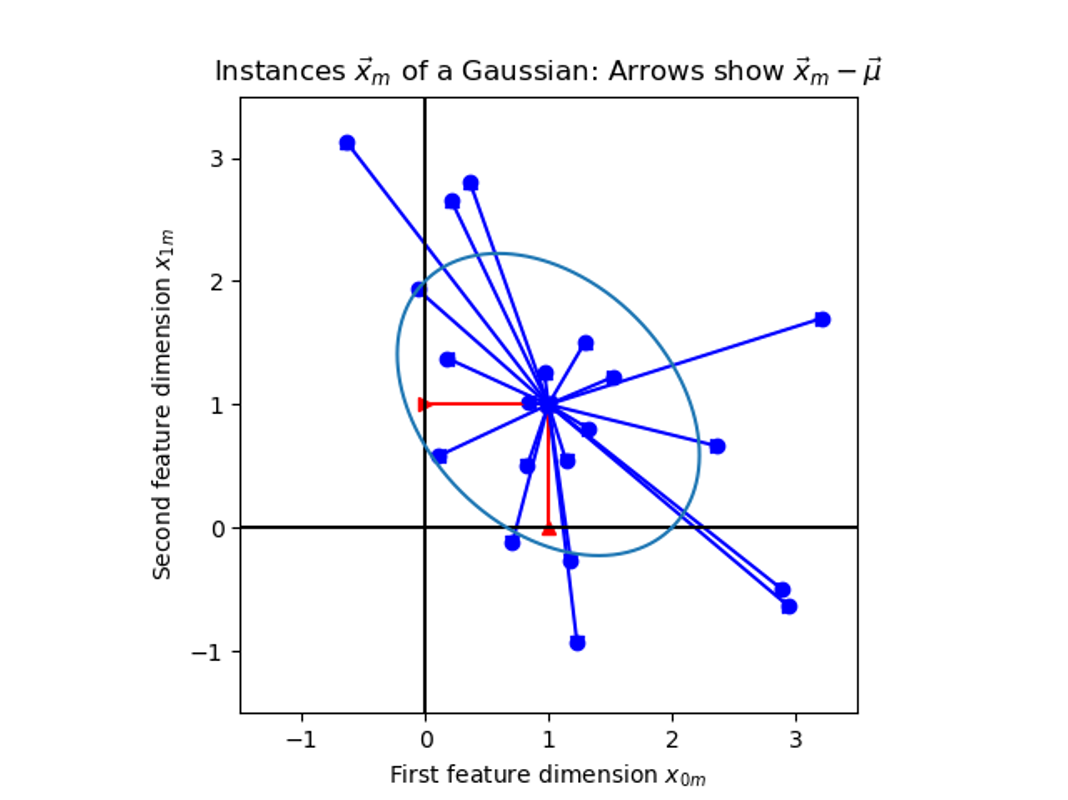
\includegraphics[width=2.1in]{gaussian_subtraction.png}
    \end{block}
  \end{columns}
\end{frame}

\begin{frame}
  \begin{columns}
    \column{1.75in}
    \begin{block}{Centered data matrix}
      \[
      X=\left[\begin{array}{c}
          (\vec{x}_0-\vec\mu)^T\\\vdots\\(\vec{x}_{M-1}-\vec\mu)^T\end{array}\right]
      \]
    \end{block}
    \column{2.625in}
    \begin{block}{Examples of $\vec{x}_m-\vec\mu$}
      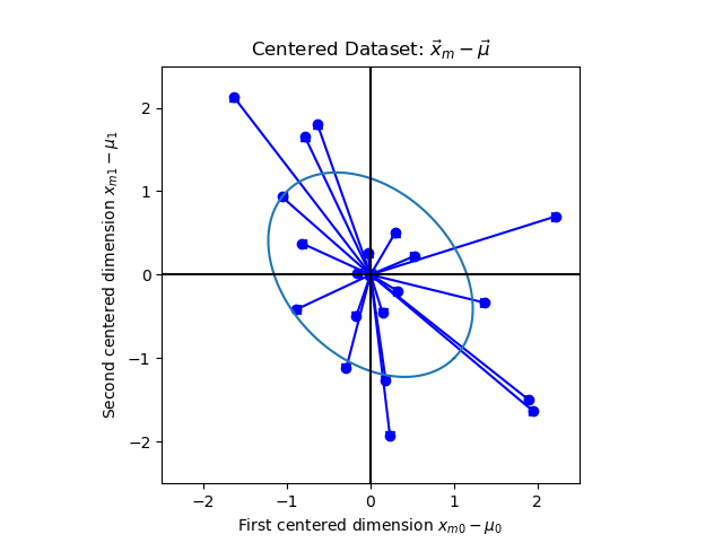
\includegraphics[width=2.5in]{centered_data.png}
    \end{block}
  \end{columns}
\end{frame}

\begin{frame}
  \begin{columns}
    \column{2.25in}
    \begin{block}{Sample covariance}
      \begin{align*}
        \Sigma&=\frac{1}{M-1}X^TX
      \end{align*}
      The matrix $X^TX$ is called the {\bf sum-of-squares (SS)} matrix.  It
      is related to the {\bf sample covariance} matrix by a scalar
      multiplier ($M-1$).
    \end{block}
    \column{2.125in}
    \begin{block}{Examples of $\vec{x}_m-\vec\mu$}
      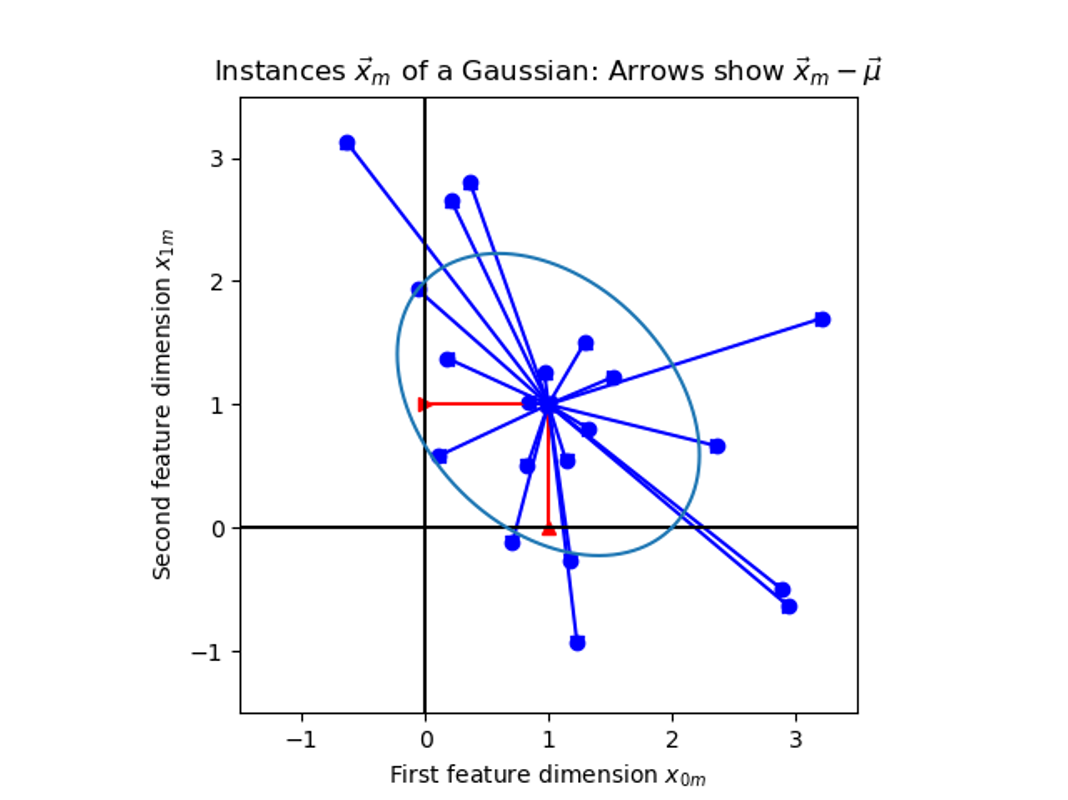
\includegraphics[width=2.1in]{gaussian_subtraction.png}
    \end{block}
  \end{columns}
\end{frame}

\begin{frame}
  \begin{columns}
    \column{1.75in}
    \begin{block}{Principal component axes}
      $X^TX$ is symmetric!  Therefore,
      \[
      X^TX=V\Lambda V^T
      \]
      $V=[\vec{v}_0,\ldots,\vec{v}_{D-1}]$, the eigenvectors
      of $X^TX$, are called the principal component axes,
      or principal component directions.
    \end{block}
    \column{2.625in}
    \begin{block}{Principal component axes}
      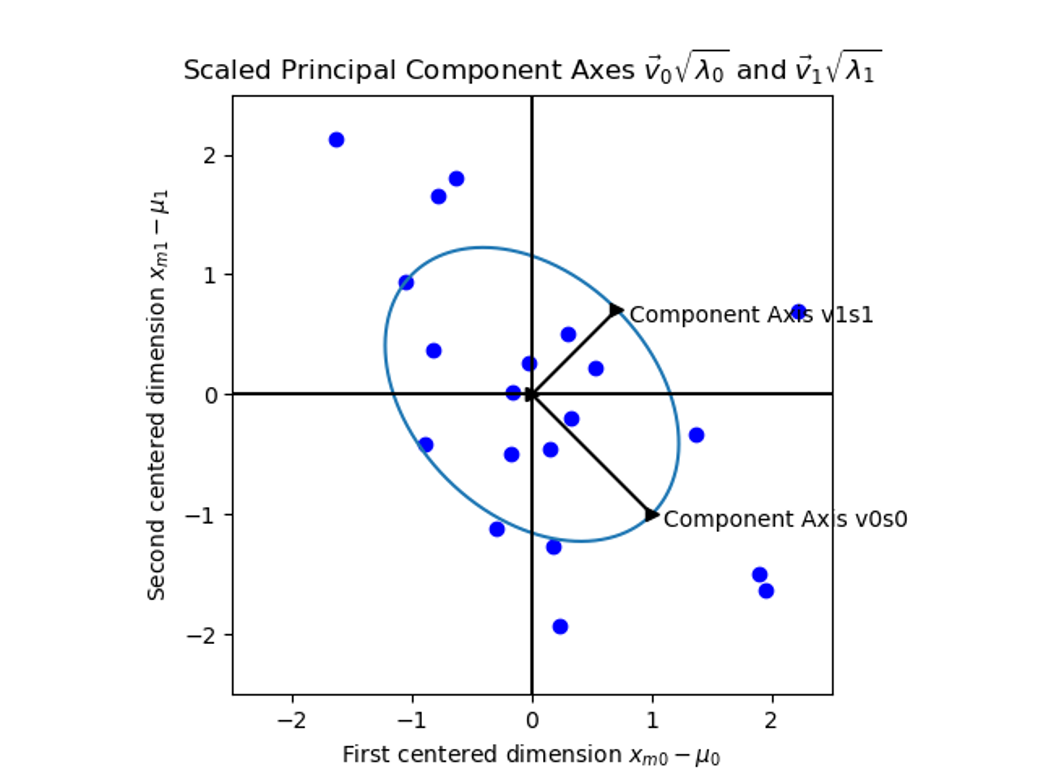
\includegraphics[width=2.5in]{principal_component_axes.png}
    \end{block}
  \end{columns}
\end{frame}

\begin{frame}
  \begin{columns}
    \column{1.75in}
    \begin{block}{Principal component axes}
      $\Sigma=\frac{1}{M-1}X^TX$, therefore
      \[
      \Sigma=V\left(\frac{1}{M-1}\Lambda\right) V^T
      \]
      $V=[\vec{v}_0,\ldots,\vec{v}_{D-1}]$ are the eigenvectors of
      both the {\bf sum-of-squares matrix} and the {\bf covariance
        matrix}.  $\Lambda$ are the eigenvalues of the sum-of-squares
      matrix, equal to $M-1$ times the eigenvalues of the covariance
      matrix.
    \end{block}
    \column{2.625in}
    \begin{block}{Principal component axes}
      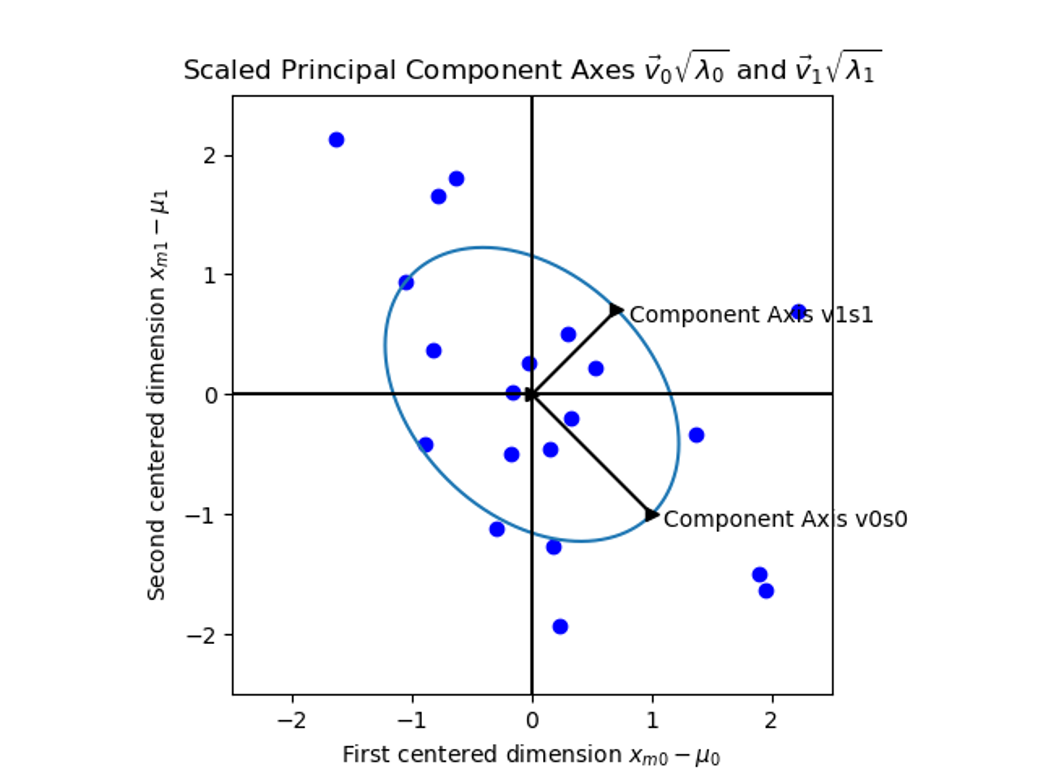
\includegraphics[width=2.5in]{principal_component_axes.png}
    \end{block}
  \end{columns}
\end{frame}

\begin{frame}
  \frametitle{Principal components}
  Remember that the eigenvectors of a matrix diagonalize it.
  So if $V$ are the eigenvectors of $X^TX$, then
  \begin{align*}
    V^TX^TXV &= \Lambda\\
    \vec{v}_i^T X^TX\vec{v}_j &= \begin{cases}
      \lambda_j & \lambda_i=\lambda_j\\
      0 & \lambda_i\ne \lambda_j
    \end{cases}
  \end{align*}
  Remember that the rows of $X$ are $(\vec{x}_m-\vec\mu)^T$, so if we
  define
  \[
  (\vec{x}_m-\vec\mu)^TV = \vec{y}_m^T,~~~~Y=
  \left[\begin{array}{c}\vec{y}_0^T\\\vdots\\\vec{y}_{M-1}^T\end{array}\right]
  \]
  Then we have that $Y^TY=\Lambda$.  In other words, the covariance
  matrix of the $\vec{y}$ vectors is a diagonal!
\end{frame}

\begin{frame}
  \frametitle{Principal components}
  \[
  \vec{y}_m=V^T(\vec{x}_m-\vec\mu)
  \]
  \centerline{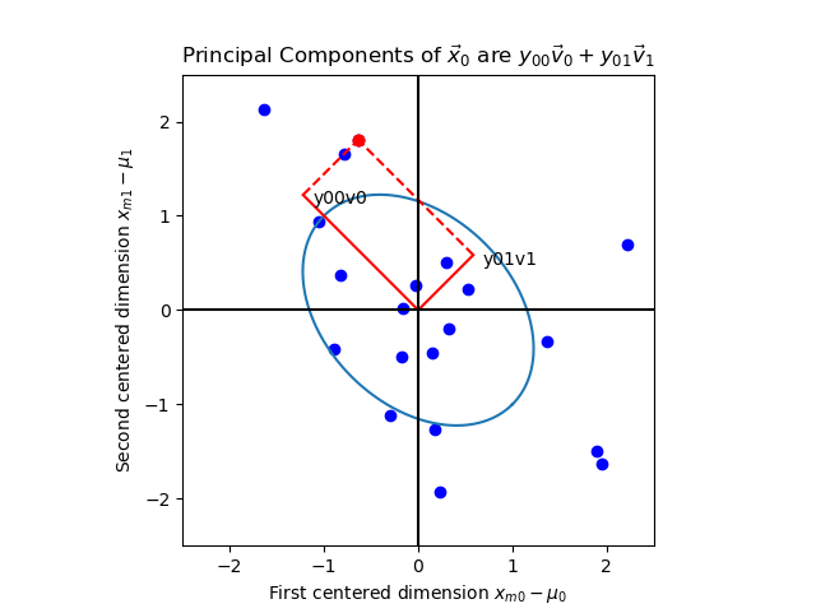
\includegraphics[height=3in]{principal_components.png}}
\end{frame}

\begin{frame}
  \frametitle{Principal components}
  Let's write $Y=XV$, and $Y^T=V^TX^T$.  In other words,
  \begin{align*}
    (\vec{x}_m-\vec\mu)^TV &= \vec{y}_m^T\\
    XV &= Y\\
    V^TX^TXV &= Y^TY  = \Lambda
  \end{align*}
  $\vec{y}_m=[y_{m,0},\ldots,y_{m,D-1}]^T$ is the vector of
  principal components of $\vec{x}_m$.  Expanding the formula
  $Y^TY=\Lambda$, we discover that PCA orthogonalizes the dataset:
  \[
  \sum_{m=0}^{M-1}y_{im}y_{jm}=\begin{cases}
  \lambda_i & i=j\\0&i\ne j
  \end{cases}
  \]
\end{frame}

\begin{frame}
  \frametitle{Principal components are uncorrelated, and PC with
    larger eigenvalues have more energy}

  In the following figure, notice that (1) the principal components
  are uncorrelated with one another, (2) the eigenvalues have been
  sorted so that $\lambda_0>\lambda_1>\lambda_2$ and so on. With this
  sorting, you see that the the first PCA, $y_{m,0}$, has the biggest
  variance:

  \centerline{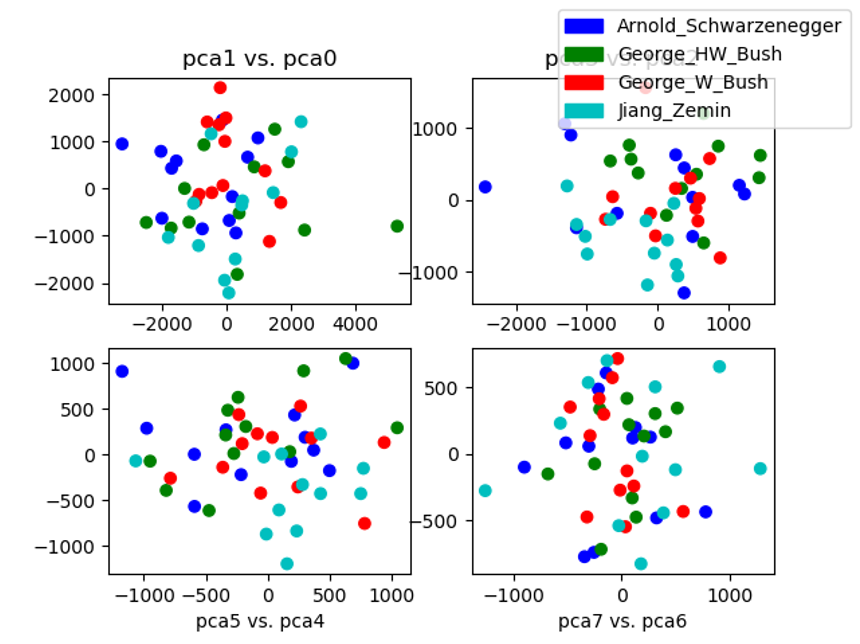
\includegraphics[height=2in]{pca_samples.png}}
\end{frame}

\begin{frame}
  \frametitle{Eigenvalue=Energy of the Principal Component} The total
  dataset energy, along the $i^{\textrm{th}}$ principal component
  direction, is
  \[
  \sum_{m=0}^{M-1}y_{mi}^2=\lambda_i
  \]
  But remember that $V^TV=I$.  Therefore, the total dataset energy
  is the same, whether you calculate it in the original image
  domain, or in the PCA domain:
  \[
  \sum_{m=0}^{M-1}\sum_{d=0}^{D-1}(x_{md}-\mu_d)^2
  =\sum_{m=0}^{M-1}\sum_{i=0}^{D-1}y_{mi}^2=\sum_{i=0}^{D-1}\lambda_i
  \]
\end{frame}

\begin{frame}
  \frametitle{Energy  spectrum=Fraction of energy explained}
  The ``energy spectrum'' is energy as a function of
  basis vector index.  There are a few ways we could define it,
  but one useful definition is:
  \begin{align*}
    E[k] &=\frac{\sum_{m=0}^{M-1}\sum_{i=0}^{k-1}y_{mi}^2}
    {\sum_{m=0}^{M-1}\sum_{i=0}^{D-1}y_{mi}^2}\\
    &=\frac{\sum_{i=0}^{k-1}\lambda_i}{\sum_{i=0}^{D-1}\lambda_i}
  \end{align*}
\end{frame}

\begin{frame}
  \frametitle{Energy  spectrum=Fraction of energy explained}
  \centerline{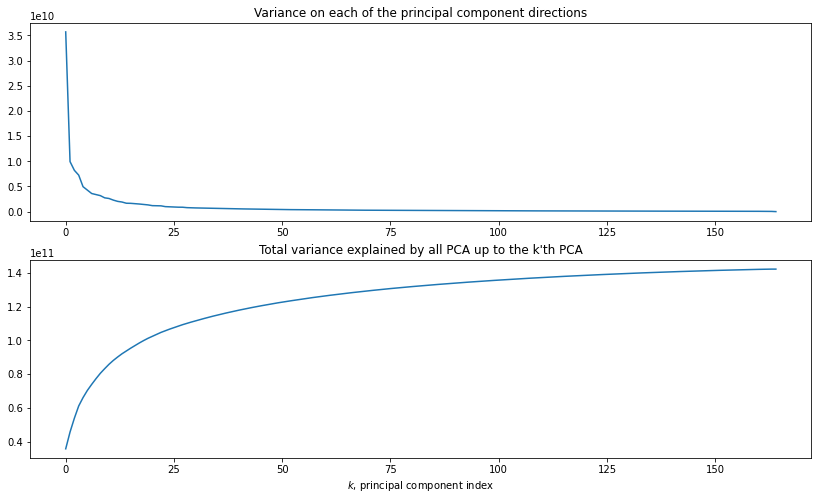
\includegraphics[height=3in]{energy_spectrum.png}}
\end{frame}


%%%%%%%%%%%%%%%%%%%%%%%%%%%%%%%%%%%%%%%%%%%%
\section[Gram]{How  to make it work: Gram matrix, SVD}
\setcounter{subsection}{1}

\begin{frame}
  \begin{columns}
    \column{2.125in}
    \begin{block}{Gram matrix}
      \begin{itemize}
      \item $X^TX$ is usually called the sum-of-squares matrix.
        $\frac{1}{M-1}X^TX$ is the sample covariance.
      \item $G=XX^T$ is called the gram matrix.
        Its $(i,j)^{\textrm{th}}$ element is the dot product between
        the $i^{\textrm{th}}$ and $j^{\textrm{th}}$ data samples:
        \[
        g_{ij}=(\vec{x}_i-\vec\mu)^T(\vec{x}_j-\vec\mu)
        \]
      \end{itemize}
    \end{block}
    \column{2.125in}
    \begin{block}{Gram matrix $g_{01}=(\vec{x}_0-\vec\mu)^T(\vec{x}_1-\vec\mu)$}
      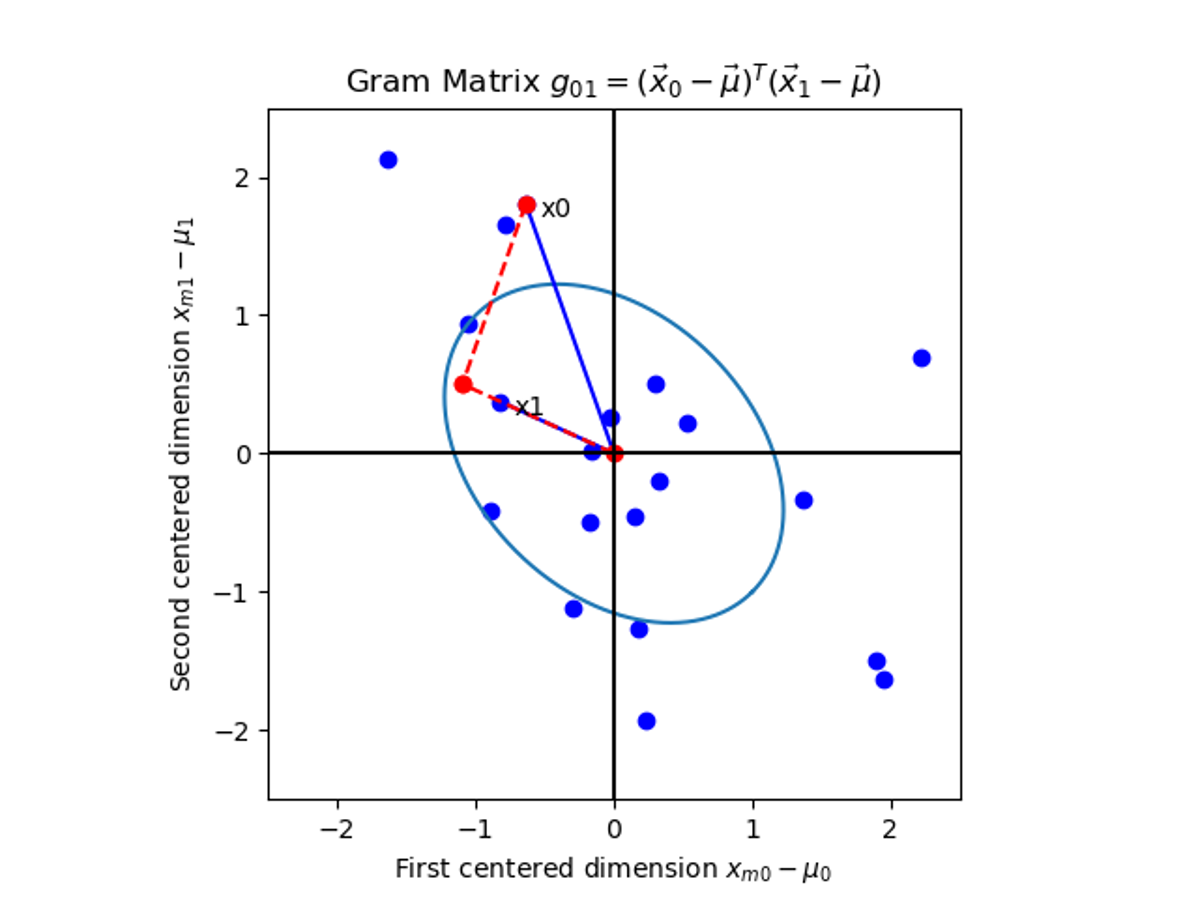
\includegraphics[width=2.1in]{gram_matrix.png}
    \end{block}
  \end{columns}
\end{frame}

\begin{frame}
  \begin{columns}
    \column{2.125in}
    \begin{block}{Eigenvectors of the Gram matrix}
      $XX^T$ is also symmetric!  So it has orthonormal eigenvectors:
      \[
      XX^T=U\Lambda U^T
      \]
      \[
      UU^T=U^TU=I
      \]
      {\bf Surprising Fact:}
      $X^TX$ and $XX^T$ have the same eigenvalues ($\Lambda$),
      but different eigenvectors ($V$ vs. $U$).
    \end{block}
    \column{2.125in}
    \begin{block}{Gram matrix $g_{01}=(\vec{x}_0-\vec\mu)^T(\vec{x}_1-\vec\mu)$}
      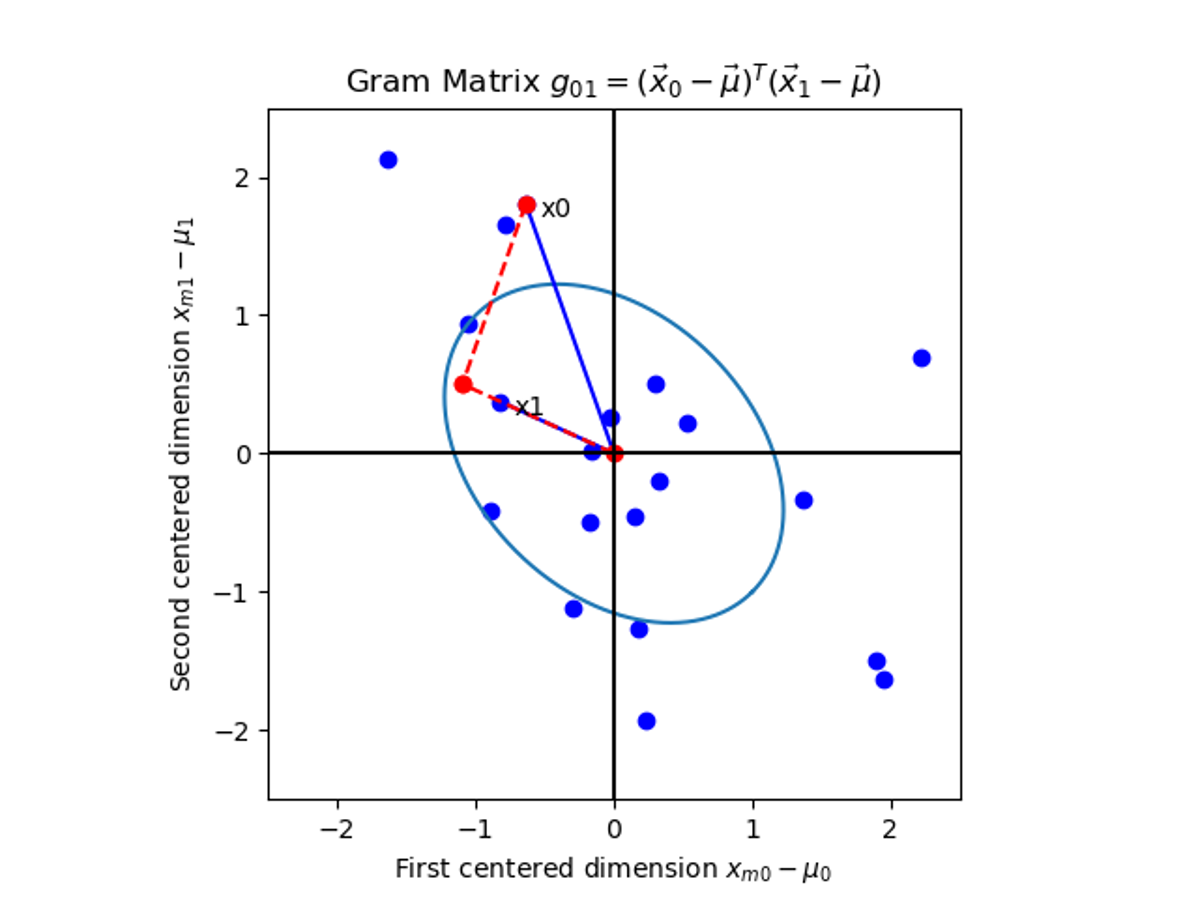
\includegraphics[width=2.1in]{gram_matrix.png}
    \end{block}
  \end{columns}
\end{frame}

\begin{frame}
  \frametitle{Why the Gram matrix is useful:}

  Suppose that $D\sim 240000$ pixels per image, but $M\sim
  240$ different images.  Then, in order to perform this eigenvalue
  analysis:
  \[
  X^TX = V\Lambda V^T
  \]
  \ldots requires factoring a $240000^{\textrm{th}}$-order polynomial
  ($|X^TX-\lambda I|=0$), then solving 240000 simultaneous linear
  equations in 240000 unknowns to find each eigenvector
  ($X^TX\vec{v}_d=\lambda_d\vec{v}_d$).  If you try doing that using
  {\tt np.linalg.eig}, your PC will be running all day.  On the other
  hand,
  \[
  XX^T=U\Lambda U^T
  \]
  requires only 240 equations in 240 unknowns.  Educated experts
  agree: $240^2 \ll 240000^2$.
\end{frame}
  
\begin{frame}
  \frametitle{Singular Values}
  \begin{itemize}
  \item Both $X^TX$ and $XX^T$ are positive semi-definite, meaning
    that their eigenvalues are non-negative, $\lambda_d\ge 0$.
  \item The {\bf singular values} of $X$ are defined to be the
    square roots of the eigenvalues of $X^TX$ and $XX^T$:
    \[
    S=\left[\begin{array}{ccc}s_0&0&0\\0&\ldots&0\\0&0&s_{D-1}\end{array}\right],~~~
    \Lambda=S^2=\left[\begin{array}{ccc}s_0^2&0&0\\0&\ldots&0\\0&0&s_{D-1}^2\end{array}\right]
    \]
  \end{itemize}
\end{frame}

\begin{frame}
  \frametitle{Singular Value Decomposition}

  Let's use the equation $\Lambda=SS$ in the PCA decomposition
  formula:
  \begin{align*}
    X^TX&= V\Lambda V^T\\
    &= VSSV^T\\
    &= VSISV^T
  \end{align*}
  \ldots where the last equation just inserted an identity matrix.  But remember, since $U$ is
  orthonormal, we can write $I=U^TU$, or
  \begin{align*}
    X^TX &= VSU^TUSV^T\\
    = (USV^T)^T(USV^T)
  \end{align*}
\end{frame}

\begin{frame}
  \frametitle{Singular Value Decomposition}

  Let's try the same thing, but starting with the Gram matrix instead:
  formula:
  \begin{align*}
    XX^T&= U\Lambda U^T\\
    &= USSU^T\\
    &= USISU^T\\
    &= USV^TVSU^T\\
    = (USV^T)(USV^T)^T
  \end{align*}
\end{frame}

\begin{frame}
  \frametitle{Singular Value Decomposition}
  {\bf ANY $M\times D$ MATRIX}, $X$, can be written as $X=USV^T$.
  \begin{itemize}
  \item $U=[\vec{u}_0,\ldots,\vec{u}_{M-1}]$ are the eigenvectors of $XX^T$.
  \item $V=[\vec{v}_0,\ldots,\vec{v}_{D-1}]$ are the eigenvectors of $X^TX$.
  \item $S=\left[\begin{array}{ccccc}s_0&0&0&0&0\\0&\ldots&0&0&0\\0&0&s_{\min(D,M)-1}&0&0\end{array}\right]$ are the singular values.
  \end{itemize}
  $S$ has some all-zero columns if $M>D$, or all-zero rows if $M<D$.
\end{frame}

\begin{frame}
  \frametitle{What np.linalg.svd does}
  First, {\tt np.linalg.svd} decides whether it wants to find the eigenvectors of
  $X^TX$ or $XX^T$: it just checks to see whether $M>D$ or vice versa.
  If it discovers that $M<D$, then:
  \begin{enumerate}
  \item Compute  $XX^T=U\Lambda U^T$, and $S=\sqrt{\Lambda}$.
    Now we have $U$ and $S$, we just need to  find $V$.
  \item Since $X^T=VSU^T$, we can get $V$ by just multiplying:
    \[
    \tilde{V} = X^TU
    \]
    \ldots where $\tilde{V}=VS$ is exactly equal to $V$, but with each column
    scaled by a different singular value.  So we just need to normalize:
    \[
    \Vert\vec{v}_i\Vert=1,~~~v_{i0}>0
    \]
  \end{enumerate}
\end{frame}

\begin{frame}
  \frametitle{Methods that solve PCA when \# faces $ll$ \# features}
  \begin{itemize}
  \item The {\bf covariance matrix} method: (eigenvector analysis of
    $X^TX$) gives the right answer, but takes {\bf a very long time}.
  \item The {\bf gram matrix} method is {\bf much faster}: Apply {\tt
    np.linalg.eig} to get $U$ from $XX^T$. Multiply $\tilde{V}=X^TU$,
    Tricky point: normalize so that $\Vert\vec{v}_k\Vert=1$,
    $v_{k,1}\ge 0$.
  \item The {\bf SVD} method: Applying {\tt np.linalg.svd(X)}.  Speed
    = {\tt min(speed(covariance),speech(gram))}.  Tricky point:
    $\lambda_m=s_m^2$.
  \end{itemize}
  Whatever you do, be sure to sort the eigenvalues so
  $|\lambda_k|\ge|\lambda_{k+1}|$.
\end{frame}

%%%%%%%%%%%%%%%%%%%%%%%%%%%%%%%%%%%%%%%%%%%%
\section[Summary]{Summary}
\setcounter{subsection}{1}

\begin{frame}
  \frametitle{Summary}
  \begin{itemize}
  \item Symmetric matrices:
    \[
    A=V\Lambda V^T,~~V^TAV=\Lambda,~~V^TV=VV^T=I
    \]
  \item Centered dataset:
    \[
    X = \left[\begin{array}{c}(\vec{x}_0-\vec\mu)^T\\\vdots\\(\vec{x}_{M-1}-\vec\mu)^T\end{array}\right]
    \]
  \item Singular value decomposition:
    \[
    X = USV^T
    \]
    where $V$ are eigenvectors of the sum-of-squares matrix, $U$ are
    eigenvectors of the gram matrix, and $\Lambda=S^2$ are their
    shared eigenvalues.
  \end{itemize}
\end{frame}

\end{document}
